\documentclass[aspectratio=169]{beamer}

\usepackage{fontspec}
\usepackage{polyglossia}
\usepackage{color}
\usepackage{listings}
\setdefaultlanguage{russian}
\usepackage{csquotes}
\usetheme{metropolis}
\metroset{background=light}
\metroset{sectionpage=none}
\metroset{numbering=fraction}

\definecolor{ssaublue}{RGB}{77,144,205}
\setbeamercolor{frametitle}{fg=white, bg=ssaublue}
\setbeamercolor{title separator}{fg=ssaublue}

\setmainfont[
    Path = ../fonts/elektratextpro/,
    Extension = .otf,
    UprightFont = elektratextpro,
    BoldFont = elektratextpro_bold,
    ItalicFont = elektratextpro_italic,
    BoldItalicFont = elektratextpro_bolditalic
]{elektratextpro}

\setsansfont[
    Path = ../fonts/elektratextpro/,
    Extension = .otf,
    UprightFont = elektratextpro,
    BoldFont = elektratextpro_bold,
    ItalicFont = elektratextpro_italic,
    BoldItalicFont = elektratextpro_bolditalic
]{elektratextpro}

\setmonofont[
    Path = ../fonts/elektratextpro/,
    Extension = .otf,
    UprightFont = elektratextpro,
    BoldFont = elektratextpro_bold,
    ItalicFont = elektratextpro_italic,
    BoldItalicFont = elektratextpro_bolditalic
]{elektratextpro}

\newfontfamily\cyrillicfont[
    Path = ../fonts/elektratextpro/,
    Extension = .otf,
    UprightFont = elektratextpro,
    BoldFont = elektratextpro_bold,
    ItalicFont = elektratextpro_italic,
    BoldItalicFont = elektratextpro_bolditalic
]{elektratextpro}

\newfontfamily\cyrillicfontsf[
    Path = ../fonts/elektratextpro/,
    Extension = .otf,
    UprightFont = elektratextpro,
    BoldFont = elektratextpro_bold,
    ItalicFont = elektratextpro_italic,
    BoldItalicFont = elektratextpro_bolditalic
]{elektratextpro}

\newfontfamily\cyrillicfonttt[
    Path = ../fonts/elektratextpro/,
    Extension = .otf,
    UprightFont = elektratextpro,
    BoldFont = elektratextpro_bold,
    ItalicFont = elektratextpro_italic,
    BoldItalicFont = elektratextpro_bolditalic
]{elektratextpro}

% Настройка листингов для Beamer
\lstset{
    basicstyle=\ttfamily\footnotesize,
    commentstyle=\color{gray},
    columns=fullflexible,
    keepspaces=true,
    breaklines=false,
    extendedchars=true,
    texcl=true,
    showstringspaces=false
}

\title{Baked Configuration + Packer}
\date{\today}

\begin{document}
    \maketitle

    \begin{frame}{Два подхода к управлению конфигурацией}
        \begin{columns}[t]
            \begin{column}[t]{0.48\textwidth}
                \textbf{Baked (образы):}
                \begin{itemize}
                    \item Заранее готовим образ с настроенным ПО
                    \item Разворачиваем готовые серверы из образа
                    \item Быстрый запуск
                \end{itemize}
                
                \vspace{0.3cm}
                \textbf{Примеры:} Docker, Packer и др.
            \end{column}
            
            \begin{column}[t]{0.48\textwidth}
                \textbf{Fry (конфигурация):}
                \begin{itemize}
                    \item Берем чистый сервер
                    \item Автоматически настраиваем его скриптами
                    \item Гибкость в настройке
                \end{itemize}
                
                \vspace{0.3cm}
                \textbf{Примеры:} Ansible, Chef, и др.
            \end{column}
        \end{columns}
        
    \end{frame}

    \begin{frame}{Baked vs Fry}
        \textbf{Плюсы baked:}
        \vspace{0.2cm}
        \begin{itemize}
            \item Предсказуемость и идентичность окружений
            \item Отсутствие configuration drift
            \item Быстрое масштабирование
        \end{itemize}

        \vspace{0.3cm}
        \textbf{Плюсы fry:}
        \vspace{0.2cm}
        \begin{itemize}
            \item Проще в настройке и поддержке
            \item Гибкость и скорость изменений
            \item Применимо к большинству приложений и серверов (в том числе к bare metal серверам)
        \end{itemize}
    \end{frame}

    \begin{frame}{От текущего к целевому состоянию}
        \begin{figure}
            \centering
            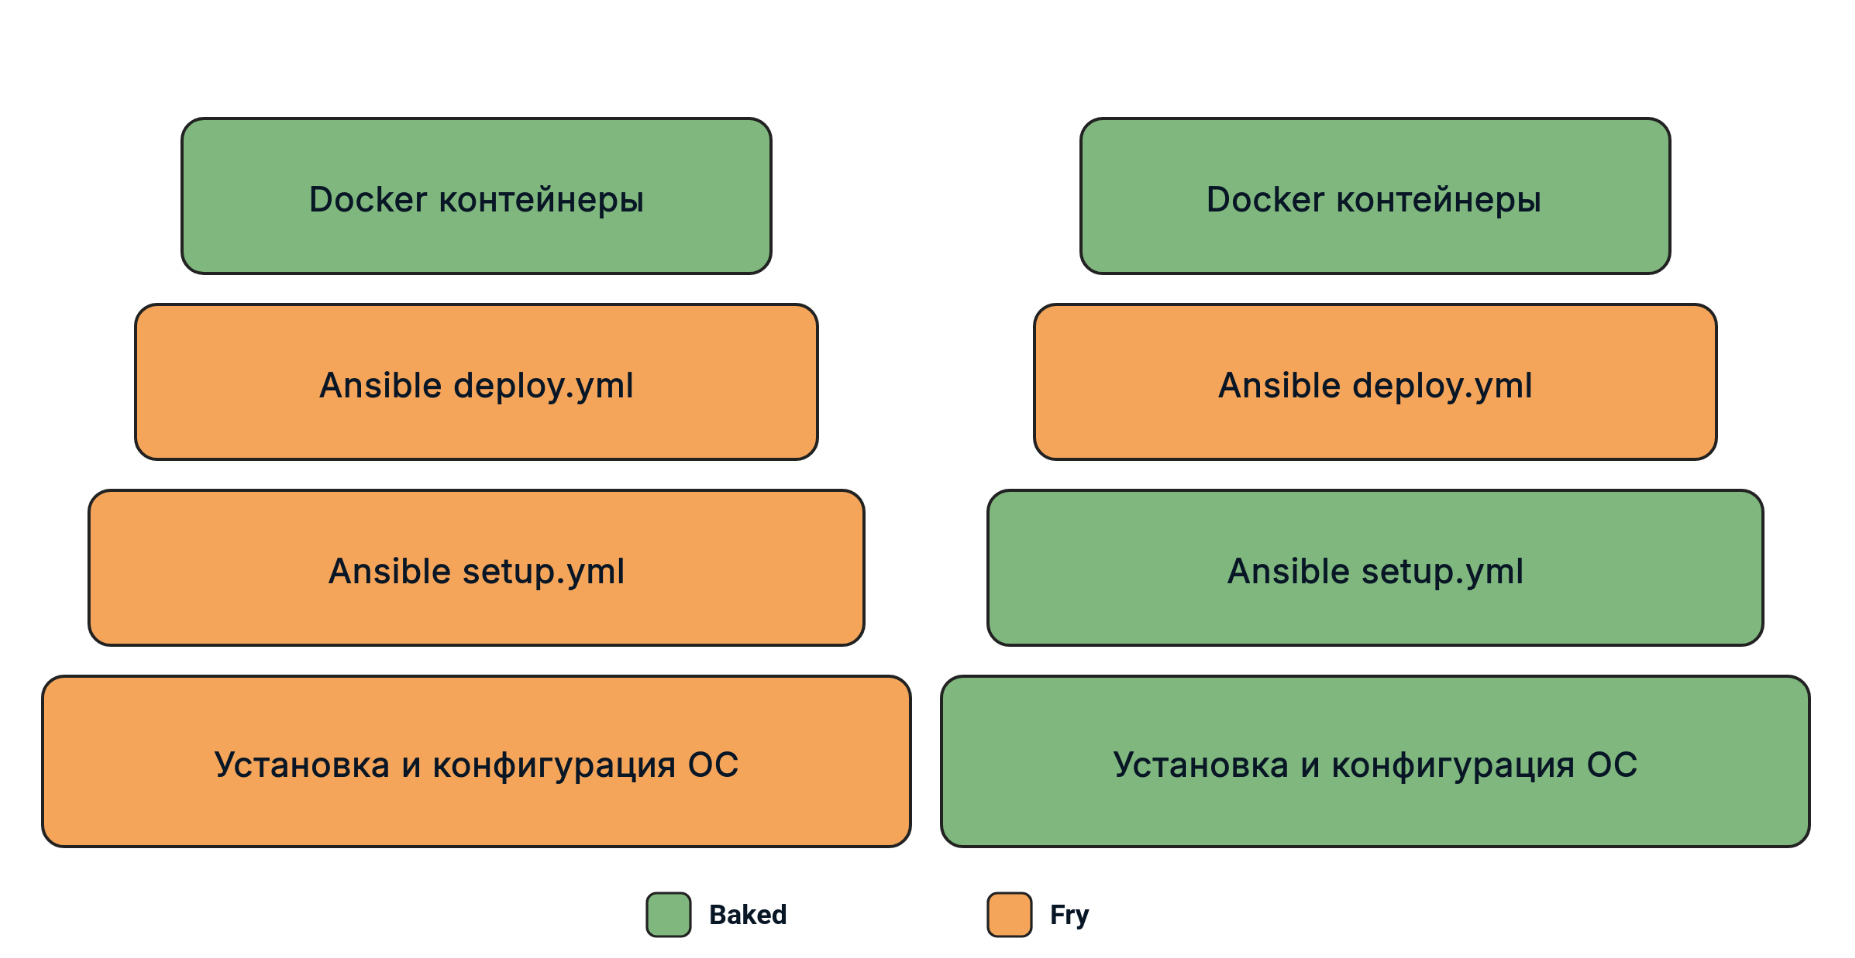
\includegraphics[width=0.9\textwidth]{media/app-before-after}
        \end{figure}
    \end{frame}

    \begin{frame}{Как реализуется baked подход?}

        \textbf{Образ} — это снимок готовой системы со всеми настройками и приложениями

        \begin{itemize}
        \item \textbf{Виртуализация}: создание образов виртуальных машин (\href{https://en.wikipedia.org/wiki/Virtual_appliance}{Virtual appliance})
        \item \textbf{Контейнеризация}: создание образов контейнеров
        \end{itemize}

        \textbf{Процесс создания образа:}
        \begin{itemize}
            \item Развертывание базового образа
            \item Настройка системы и установка ПО
            \item Сохранение итогового образа
        \end{itemize}

        \footnotesize{\textcolor{gray}{\url{https://en.wikipedia.org/wiki/Software_appliance\#Types_of_software_appliances}}}
    \end{frame}

    \begin{frame}{Демонстрация: Создание VA в VirtualBox}
        \textbf{Что покажем:}
        \begin{itemize}
            \item Ручная установка Alpine Linux в VirtualBox
            \item Ручная настройка системы, установка nginx
            \item Создание образа
        \end{itemize}
    \end{frame}

    \begin{frame}{Что такое Packer?}
        \textbf{HashiCorp Packer} — инструмент для создания идентичных машинных образов
        
        \vspace{0.5cm}
        
        \textbf{Основные возможности:}
        \begin{itemize}
            \item Автоматизация создания образов виртуальных машин
            \item Поддержка разных платформ (VirtualBox, VMware, облачные провайдеры)
            \item Разные способы настройки (Shell, Ansible)
        \end{itemize}
    \end{frame}

    \begin{frame}{Архитектура Packer}
        \textbf{Процесс создания образа:}
        
        \begin{enumerate}
            \item Packer запускает временную VM
            \item Подключается к ней по SSH
            \item Выполняет скрипты установки и настройки
            \item Создает образ из настроенной VM
            \item Удаляет временную VM
        \end{enumerate}
        
        \vspace{0.5cm}
        
        \textbf{Компоненты Packer:}
        \begin{itemize}
            \item \textbf{Builder} — создает VM (virtualbox, vmware, облачные)
            \item \textbf{Provisioner} — настраивает VM (shell, ansible)
            \item \textbf{Template} — HCL файл с описанием процесса
        \end{itemize}
    \end{frame}

    \begin{frame}{Демонстрация: Packer + VirtualBox}
        \textbf{Что покажем:}
        \begin{itemize}
            \item Написание Packer template для VirtualBox
            \item Миграция настроек из демки с Virtual Appliance
            \item Создание образа с предустановленным nginx
            \item Автоматизация процесса создания образов
            \item Сравнение времени: ручная настройка vs Packer
        \end{itemize}

        \vspace{0.2cm}
        \textbf{Демо-репозиторий:} \\
        \href{https://github.com/prafdin/devops-demo-website/tree/packer-demo}{\texttt{https://github.com/prafdin/devops-demo-website/tree/packer-demo}}
    \end{frame}

    \begin{frame}{Что запомнить}
        \begin{itemize}
            \item \textbf{Packer} позволяет описать создание образа VM через код
            \item \textbf{Virtual Appliance} — готовые образы виртуальных машин
            \item \textbf{Immutable Infrastructure} — образы не изменяются, только заменяются
        \end{itemize}

        \vspace{1cm}

        \begin{center}
            \textbf{Вопросы?}
        \end{center}
    \end{frame}

\end{document}